\documentclass{standalone}
\usepackage{tikz}

\usetikzlibrary{automata,positioning,arrows,shapes,decorations,calc,
arrows.meta,fit}
\usetikzlibrary{decorations.pathmorphing}
\usetikzlibrary{decorations.pathreplacing}
\usetikzlibrary{decorations.shapes}
\usetikzlibrary{decorations.text}
\usetikzlibrary{decorations.markings}
\usetikzlibrary{decorations.fractals}
\usetikzlibrary{decorations.footprints}

\tikzset{
roundnode/.style={circle, draw=black, very thick, minimum size=20mm},
>={Latex[width=2mm,length=2mm]},
goal/.style={circle, double, draw=black, very thick, minimum size=20mm},
simple/.style={circle, draw=black, very thick, minimum size=20mm},
table/.style={circle, draw=black, very thick, minimum size=20mm, fill=lightgray},
screen/.style={circle, draw=black, very thick, minimum size=20mm, fill=green},
>={Latex[width=2mm,length=2mm]},
base/.style = {rectangle, rounded corners, draw=black,
                         minimum width=4cm, minimum height=1cm,
                         text centered, font=\sffamily},
}

\begin{document}
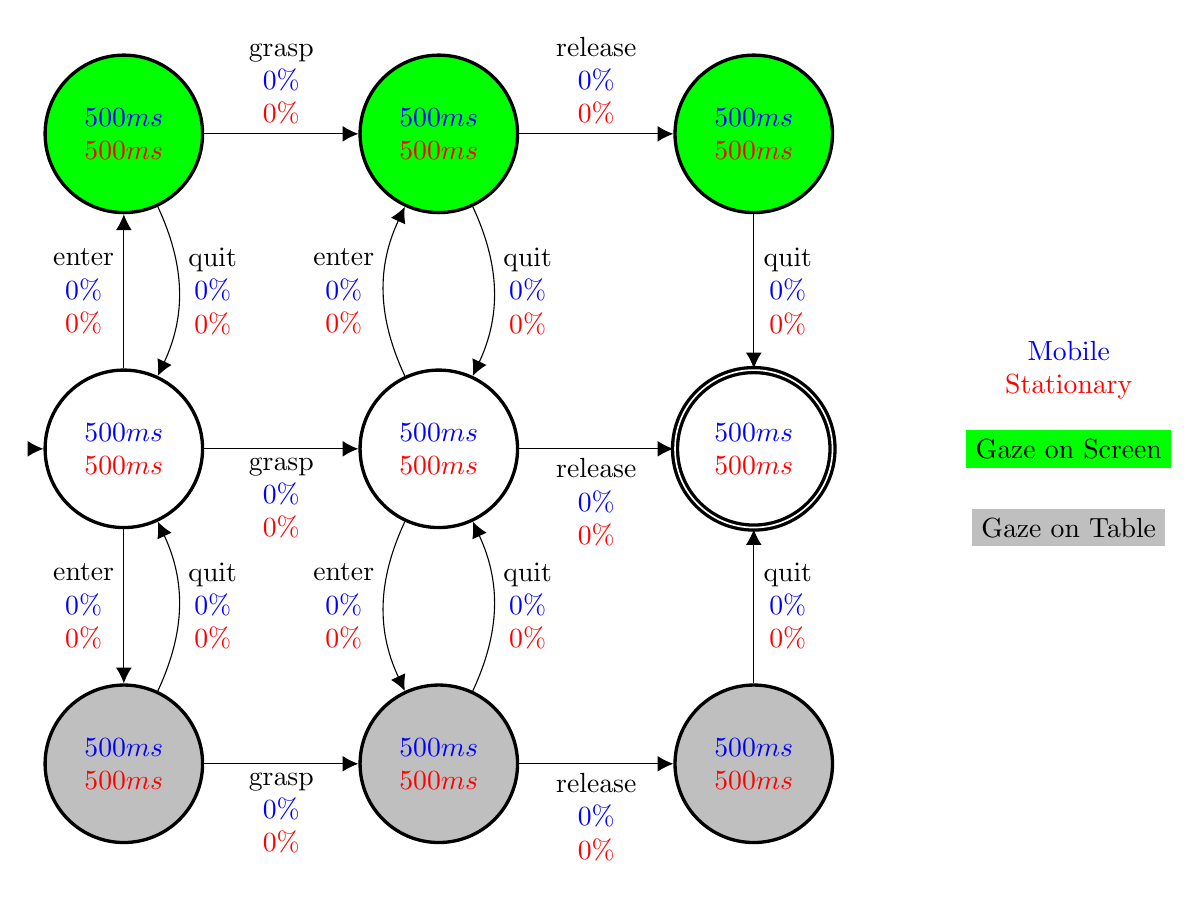
\begin{tikzpicture}[node distance=5cm, align=center]

    \node (start) at(19,-15)  {};

    \node[rectangle] (leg1) at(32, -14)  {\textcolor{blue}{Mobile}\\\textcolor{red}{Stationary}};
    \node[rectangle,fill=green] (leg1) at(32, -15)  {Gaze on Screen};
    \node[rectangle,fill=lightgray] (leg1) at(32, -16)  {Gaze on Table};

    \node[simple] (n0) at(20, -15)  {\textcolor{blue}{$500ms$}\\\textcolor{red}{$500ms$}};
    \node[simple] (n3) at(24, -15)  {\textcolor{blue}{$500ms$}\\\textcolor{red}{$500ms$}};

    \node[goal] (n6) at(28, -15)  {\textcolor{blue}{$500ms$}\\\textcolor{red}{$500ms$}};

    \node[table] (n1) at(20, -19)  {\textcolor{blue}{$500ms$}\\\textcolor{red}{$500ms$}};
    \node[table] (n4) at(24, -19)  {\textcolor{blue}{$500ms$}\\\textcolor{red}{$500ms$}};
    \node[table] (n7) at(28, -19)  {\textcolor{blue}{$500ms$}\\\textcolor{red}{$500ms$}};

    \node[screen] (n2) at(20, -11)  {\textcolor{blue}{$500ms$}\\\textcolor{red}{$500ms$}};
    \node[screen] (n5) at(24, -11)  {\textcolor{blue}{$500ms$}\\\textcolor{red}{$500ms$}};
    \node[screen] (n8) at(28, -11)  {\textcolor{blue}{$500ms$}\\\textcolor{red}{$500ms$}};

    \draw[->] (start)  to (n0) ;

    \draw[->] (n0)  to node[left] {enter\\\textcolor{blue}{$0\%$}\\\textcolor{red}{$0\%$}} (n1) ;
    \draw[->] (n0)  to node[left] {enter\\\textcolor{blue}{$0\%$}\\\textcolor{red}{$0\%$}} (n2) ;

    \draw[->] (n1)  to [bend right=25] node[right] {quit\\\textcolor{blue}{$0\%$}\\\textcolor{red}{$0\%$}} (n0) ;
    \draw[->] (n2)  to [bend left=25] node[right] {quit\\\textcolor{blue}{$0\%$}\\\textcolor{red}{$0\%$}} (n0) ;

    \draw[->] (n0)  tonode[below] {grasp\\\textcolor{blue}{$0\%$}\\\textcolor{red}{$0\%$}} (n3) ;
    \draw[->] (n1)  tonode[below] {grasp\\\textcolor{blue}{$0\%$}\\\textcolor{red}{$0\%$}} (n4) ;
    \draw[->] (n2)  tonode[above] {grasp\\\textcolor{blue}{$0\%$}\\\textcolor{red}{$0\%$}} (n5) ;

    \draw[->] (n8)  to node[right] {quit\\\textcolor{blue}{$0\%$}\\\textcolor{red}{$0\%$}} (n6) ;
    \draw[->] (n7)  to node[right] {quit\\\textcolor{blue}{$0\%$}\\\textcolor{red}{$0\%$}} (n6) ;

    \draw[->] (n3)  to node[below] {release\\\textcolor{blue}{$0\%$}\\\textcolor{red}{$0\%$}} (n6) ;
    \draw[->] (n4)  to node[below] {release\\\textcolor{blue}{$0\%$}\\\textcolor{red}{$0\%$}} (n7) ;
    \draw[->] (n5)  to node[above] {release\\\textcolor{blue}{$0\%$}\\\textcolor{red}{$0\%$}} (n8) ;

    \draw[->] (n4)  to [bend right=25] node[right] {quit\\\textcolor{blue}{$0\%$}\\\textcolor{red}{$0\%$}} (n3) ;
    \draw[->] (n5)  to [bend left=25] node[right] {quit\\\textcolor{blue}{$0\%$}\\\textcolor{red}{$0\%$}} (n3) ;

    \draw[->] (n3)  to [bend right=25] node[left] {enter\\\textcolor{blue}{$0\%$}\\\textcolor{red}{$0\%$}} (n4) ;
    \draw[->] (n3)  to [bend left=25] node[left] {enter\\\textcolor{blue}{$0\%$}\\\textcolor{red}{$0\%$}} (n5) ;




\end{tikzpicture}
\end{document}
